%\documentclass{exam}
\documentclass[answers,addpoints]{exam}
\usepackage{amsmath,amssymb,enumerate,float,tikz,etoolbox,ifthen,xcolor,ulem,graphicx, comment,hyperref,multicol,enumerate,makecell,pgfplots,geometry}
\pgfplotsset{compat=1.18}
\usetikzlibrary{decorations.pathreplacing}

\geometry{
  % margin=1in,
  top=0.5in,
  bottom=0.5in,
  left=0.75in,
  right=0.75in,
  letterpaper
}

\definecolor{MyGreen}{rgb}{0.1, 0.4, 0.1}
\definecolor{MyBlue}{rgb}{0.1, 0.1, 0.9}

\AtBeginEnvironment{solution}{\color{MyGreen}}

\newboolean{NoSolutions}

\newcommand\pts[1][2]{\textcolor{MyBlue}{\text{\bf [#1 pts]}}}
\newcommand\pt{\textcolor{MyBlue}{\text{\bf [1 pt]}}}
\newcommand\ds{\displaystyle}

\makeatletter
\renewcommand{\thefigure}{\thequestion.\arabic{figure}}
\@addtoreset{figure}{question}
\makeatother

\setlength\parindent{0in}
\pagestyle{empty}
\begin{document}

\section*{MATH 100 GROUP PROJECT 2: \\Implicit Differentiation and Linear Approximation}

\normalsize

\subsection*{Contributors}

Alexandre \textbf{Boutoille} (22291660) Brennan \textbf{Coetzer} (64702178) Dino \textbf{Lee} (29709300) Andaya \textbf{Vincent} (33234436)

\hrulefill

\subsection*{Reflection Question}

\begin{solution}
  The questions in high school math are more directed towards solving problems using equations and following steps taught in class, whereas the questions in the first group project require a lot more thought and proof, both in mathematical equations, graphs, and especially written explanations. This requires a much deeper understanding of different mathematical concepts rather than just how to apply them.

  Currently Group 6 communicates well on Instagram, as everyone monitors the group chat closely for information and questions about delegated tasks and meetings. Currently, some members have contributed more to the initial steps in problem-solving, while others contribute to the later and final steps of the project. Ideally, all members will contribute to all stages of the process. To even the workload, the group will try to set up a meeting before working on the project to make sure everyone is on the same page. After that, subsequent meetings may potentially be helpful to complete group work or not, depending on the group consensus. It may be that if a person completes more tasks, they may have more flexibility for attending an upcoming meeting than someone who has completed fewer tasks to balance out the workload.
\end{solution}

\hrulefill

\newpage

\fullwidth{
\subsection*{Assignment questions}}

\begin{questions}
  \question \
  \begin{solution}

    \begin{figure}[H]
      \centering
      \begin{tabular}{@{}l@{}}
        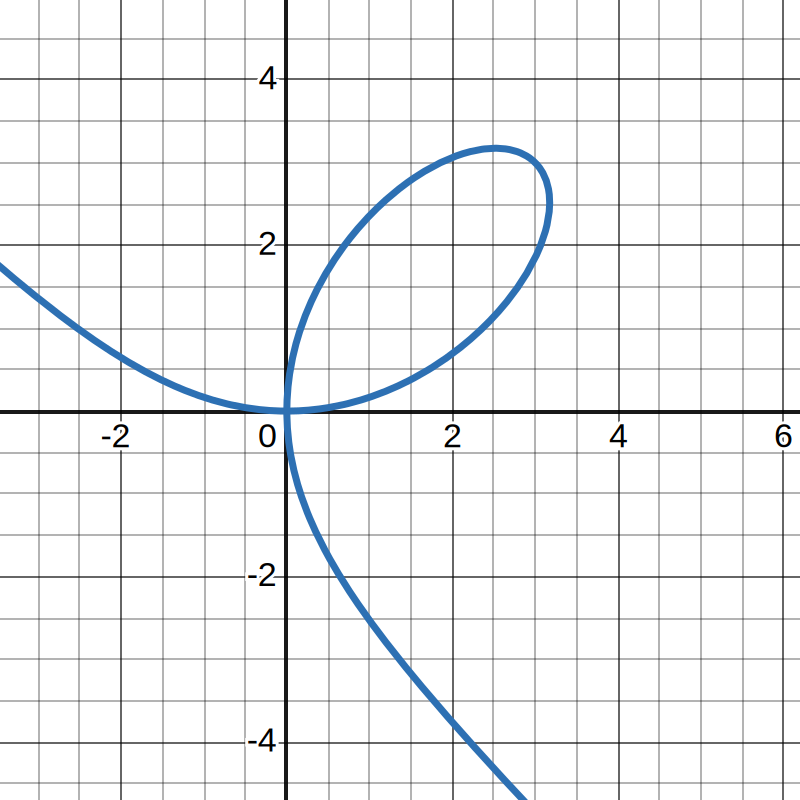
\includegraphics[width=5cm]{desmos-graph.png}
      \end{tabular}
      \caption{$x^3+y^3=6xy$ Graph}
      \label{fig:graph}
    \end{figure}

    \begin{figure}[H]
      \centering
      \begin{tabular}{@{}l@{}}
        $\displaystyle x^3+y^3=6xy$ \\[6pt]
        $\displaystyle (3)^3+(3)^3=6(3)(3)$ \\[6pt]
        $\displaystyle 54=54$ \\[12pt]
        $\displaystyle \frac{d}{dx}3x^2+\frac{dy}{dx}3y^2=\frac{d}{dx}6y+\frac{dy}{dx}6x$ \\[6pt]
        $\displaystyle \frac{dy}{dx}=\frac{2y-x^2}{y^2-2x}$ \\[6pt]
        $\displaystyle \frac{dy}{dx}=\frac{2(3)-(3)^2}{(3)^2-2(3)}$ \\[6pt]
        $\displaystyle =-1$ \\[12pt]
        $\displaystyle L(x)=f(a)+f^\prime(x)(x-a)$ \\[6pt]
        $\displaystyle L(x)=(3)+(-1)(x-3)$ \\[6pt]
        $\displaystyle y=-x+6$ \\
      \end{tabular}
      \caption{1a Mathematical Work}
      \label{fig:1a-math}
    \end{figure}

    It is assumed that $y=f(x)$ if $(3,3)$ exists and has only one tangent line. Although $x=3$ has two values as seen in \ref{fig:graph}, $y=f(x)$ exists locally at $(3,3)$. If $y=f(x)$ could not be written at the point, the tangent line would not exist with a value of $\infty$. This would indicate a graph turning-back on itself Even though the curve fails the VLT, there is only one tangent line in the small region. Therefore, the slope is $-1$—a real number—so $y=f(x)$ near $(3,3)$.

    \begin{figure}[H]
      \centering
      \begin{tabular}{@{}l@{}}
        $\displaystyle L(x)=f(a)+f^\prime(a)(x-a)$ \\[6pt]
        $\displaystyle L(1)=3-1(1-3)$ \\[6pt]
        $\displaystyle L(2.5)=3-1(2.5-3)$ \\[6pt]
        $\displaystyle =3.5$ \\
      \end{tabular}
      \caption{1b Mathematical Work}
      \label{fig:1b-math}
    \end{figure}

    The single-step estimate $b$ is inaccurate, as linear approximations are accurate the more you deviate from where the approximation was derived from. Linear approximations find points on a tangent line; hence, the further you deviate, the more accuracy decreases. Regardless, since the curve is concave downwards as seen in \ref{fig:graph}, the real value at $x=2.5$ will be less than the overestimate provided by the approximation.

  \end{solution}

  % -------------------------------------------------------

  \question \
  \begin{solution}

    \begin{figure}[H]
      \centering
      \begin{tabular}{r r r r r r}
        \hline
        \multicolumn{1}{c}{$n$} &
        \multicolumn{1}{c}{$x_n$} &
        \multicolumn{1}{c}{$y_n$} &
        \multicolumn{1}{c}{$m_n$} &
        \multicolumn{1}{c}{$x_{n+1}$} &
        \multicolumn{1}{c}{$y_{n+1}$} \\
        \hline
        0 & 3.0000 & 3.0000 & -1.0000 & 2.9000 & 3.1000 \\
        1 & 2.9000 & 3.1000 & -0.5801 & 2.8000 & 3.1580 \\
        2 & 2.8000 & 3.1580 & -0.3485 & 2.7000 & 3.1929 \\
        3 & 2.7000 & 3.1929 & -0.1886 & 2.6000 & 3.2117 \\
        4 & 2.6000 & 3.2117 & -0.0658 & 2.5000 & 3.2183 \\
        5 & 2.5000 & 3.2183 & 0.0348 & 2.4000 & 3.2148 \\
        \hline
      \end{tabular}
      \caption{2a Calculations Table}
      \label{fig:2a-vi-table}
    \end{figure}

    \begin{figure}[H]
      \centering
      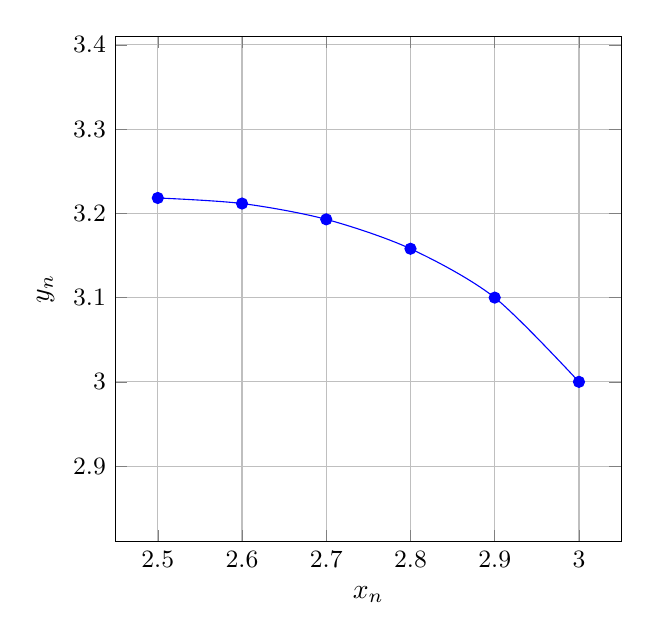
\begin{tikzpicture}
        \begin{axis}[
            axis equal,
            xlabel=$x_n$,
            ylabel=$y_n$,
            grid=both,
            width=8cm,
            height=8cm,
            xmin=2.45, xmax=3.05,
            ymin=3.0, ymax=3.22,
            tick label style={font=\small}
          ]

          \addplot[blue, mark=*,thin,smooth] coordinates {
            (3.0000, 3.0000)
            (2.9000, 3.1000)
            (2.8000, 3.1580)
            (2.7000, 3.1929)
            (2.6000, 3.2117)
            (2.5000, 3.2183)
          };
        \end{axis}
      \end{tikzpicture}
      \caption{2a $x_n$ vs $y_n$ plot}
      \label{fig:2a-vii-plot}
    \end{figure}

    The new $b$ value of $b \approx 3.218927$ is closer than the value of $3.5$ obtained in \ref{fig:1a-math}. The increased accuracy comes from the addition of a new tangent line every time we move close to $2.5$ from $3$. However, since values of $y_n+1$ are approximated using $m_n$, the tangent line overshoots the actual value(s) of the curve. These errors accumulate, resulting in an over-approximated value of $b$.

    \begin{figure}[H]
      \centering
      \begin{tabular}{r r r r r r}
        \hline
        \multicolumn{1}{c}{$n$} &
        \multicolumn{1}{c}{$x_n$} &
        \multicolumn{1}{c}{$y_n$} &
        \multicolumn{1}{c}{$m_n$} &
        \multicolumn{1}{c}{$x_{n+1}$} &
        \multicolumn{1}{c}{$y_{n+1}$} \\
        \hline
        0 & 3.0000 & 3.0000 & -1.0000 & 2.9500 & 3.0500 \\
        1 & 2.9500 & 3.0500 & -0.7649 & 2.9000 & 3.0882 \\
        2 & 2.9000 & 3.0882 & -0.5976 & 2.8500 & 3.1181 \\
        3 & 2.8500 & 3.1181 & -0.4689 & 2.8000 & 3.1416 \\
        4 & 2.8000 & 3.1416 & -0.3646 & 2.7500 & 3.1598 \\
        5 & 2.7500 & 3.1598 & -0.2772 & 2.7000 & 3.1737 \\
        6 & 2.7000 & 3.1737 & -0.2018 & 2.6500 & 3.1837 \\
        7 & 2.6500 & 3.1837 & -0.1354 & 2.6000 & 3.1905 \\
        8 & 2.6000 & 3.1905 & -0.0761 & 2.5500 & 3.1943 \\
        9 & 2.5500 & 3.1943 & -0.0223 & 2.5000 & 3.1954 \\
        10 & 2.5000 & 3.1954 & 0.0270 & 2.4500 & 3.1941 \\
        \hline
      \end{tabular}
      \caption{2b Calculations Table}
      \label{fig:2b-table}
    \end{figure}

    \begin{figure}[H]
      \centering
      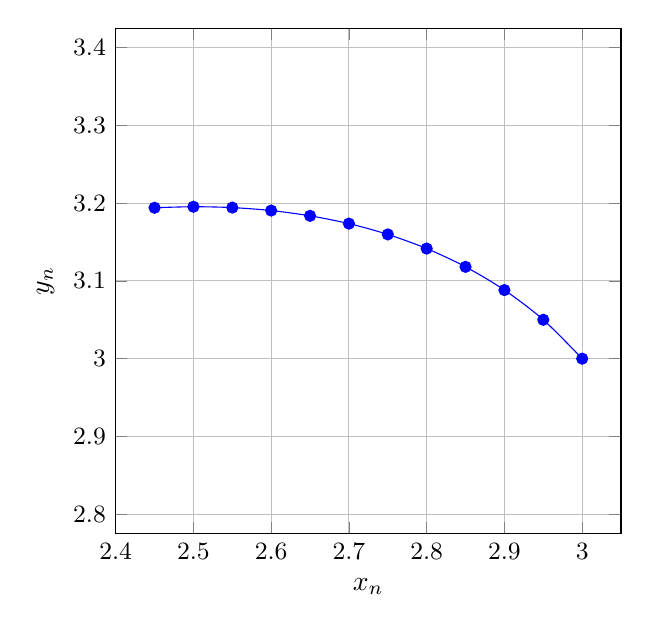
\begin{tikzpicture}
        \begin{axis}[
            axis equal,
            xlabel=$x_n$,
            ylabel=$y_n$,
            grid=both,
            width=8cm,
            height=8cm,
            xmin=2.40, xmax=3.05,
            ymin=3.0, ymax=3.20,
            tick label style={font=\small}
          ]

          \addplot[blue, mark=*,thin,smooth] coordinates {
            (3.0000, 3.0000)
            (2.9500, 3.0500)
            (2.9000, 3.0882)
            (2.8500, 3.1181)
            (2.8000, 3.1416)
            (2.7500, 3.1598)
            (2.7000, 3.1737)
            (2.6500, 3.1837)
            (2.6000, 3.1905)
            (2.5500, 3.1943)
            (2.5000, 3.1954)
            (2.4500, 3.1941)
          };
        \end{axis}
      \end{tikzpicture}
      \caption{2b $x_n$ vs $y_n$ plot}
      \label{fig:2b-plot}
    \end{figure}

    Changing $h$ from $0.1$ to $0.05$ change the approximation to $b \approx 3.195442$. This is closer to the actual value of $b \approx 3.174607$, meaning a smaller $h$ improves the approximation accuracy. This is because calculating values of $y_n$ more frequently with smaller $h$ values creates tangent lines closer to the curve with less error. This results in a curve for \ref{fig:2b-plot} more accurate to the actual value of $b$.

  \end{solution}

  %\hrulefill
  % -------------------------------------------------------
  \question \
  \begin{solution}

    \begin{figure}[H]
      \centering
      \begin{tabular}{@{}l@{}}
        $\displaystyle \frac{dy}{dx}=\frac{2(0)-(0^2)}{(0)^2-2(0)}$ \\[6pt]
        $\displaystyle =0=\text{DNE}$ \\[6pt]
      \end{tabular}
      \caption{3a Mathematical Work}
      \label{fig:3a-math}
    \end{figure}

    As seen in \ref{fig:graph}, multiple paths pass through $(0,0)$. It is a point of self-intersection with no well-defined tangent direction. Therefore, the tangent line method cannot be used reliably. The derivative found in \ref{fig:1a-math} cannot be simplified at $(0,0)$ using L'Hôpital's rule, as seen in \ref{fig:3a-math}. Therefore, a slope cannot be obtained for the tangent line, so the iterative tangent line method at $(0,0)$ cannot be used.

    A linear approximation cannot be used to find $(p,q)$ when $q=1$ at $(0,0)$. This is because the slope of the tangent line is an indeterminate form, as there is an intersection of paths at $(0,0)$ on the graph. We cannot use iterative tangent line techniques to estimate anything starting at $(0,0)$, as the initial slope is an indeterminate form.

    Since there is no singular tangent line exists at $(0,0)$ when the graph intersects, as there are multiple paths leading to $(0,0)$, problems will arise when solving for the slope, as seen in \ref{fig:3a-math}.

    There are multiple tangent lines at $(0,0)$. This suggests there are multiple coordinates that the linear approximation could give at this point for $(a,b)$ when $a=1$, and $(p,q)$ with $q=1$. Generally, this approach cannot be applied starting at $(0,0)$.

    \begin{figure}[H]
      \centering
      \begin{tabular}{@{}l@{}}
        $\displaystyle m_0\frac{2(0)^2-(0.05)^2}{(0)^2-2(0.05)}=0.025$ \\[6pt]
        $\displaystyle x_1=(0.05)+(0.05)=0.1$ \\[6pt]
        $\displaystyle y_1=0+(0.05)(0.025)=0.00125$ \\[6pt]
        $\displaystyle (x_1,y_1)=(0.1,0.00125)$ \\[6pt]
        $\displaystyle m_1\frac{2(0.00125)-(0.1)^2}{(0.00125)^2-2(0.1)}=0.037500293...$ \\[6pt]
        $\displaystyle x_2=0.15$ \\[6pt]
        $\displaystyle y_2=3.125014659...\cdot10^{-3}$ \\[6pt]
        $\displaystyle (x_2,y_2)=(0.15,0.003123015...)$ \\[6pt]
        $\displaystyle $ \\[6pt]
      \end{tabular}
      \caption{3d Mathematical Work}
      \label{fig:3d-math}
    \end{figure}

    The intermediate means $(0,0)$ cannot be used as a starting point, but $(0.05,0)$—a nearby point—can be used. The true $y$-value at $x=0.05$ is unknown, but is approximated to be near $0$. Using $(x_0,y_0)$, the iterative line approach can be used in small increments of $h=0.05$ for accurate tangent line points near $(0,0)$. \ref{fig:3d-math} demonstrates the steps to solve for a tangent line near $(0,0)$. This provides a good approximation of values to overcome the issues when starting at $(0,0)$. At $(0,0)$, the points intersect perfectly, but not at points near $(0,0)$—the iterative method can be used there. To find an estimate of an $x$-value of $1$, the iterative process could be continued until an $x$-value of $1$ is reached.

    To increase the mathematical approach's accuracy, $h$ could be incremented in smaller steps with diminishing returns. In theory, the most accurate increment would be values infinitely close to $0$, all the way to the desired value, as there would be an infinite amount of linear approximations. This would preset a perfectly accurate value at any point. In practice, this approach would be ineffective as it would take an infinite amount of time to calculate. The core concept is that smaller $h$ increments produces smaller changes in $x$ and $y$ values resulting in approximations closer to the curve. This gives the most accurate final value, but takes more steps.

  \end{solution}

  % -------------------------------------------------------

  \hrulefill
  % -------------------------------------------------------

  % -------------------------------------------------------

\end{questions}
\end{document}

%-------------------------------------------------------------
%-------------------------------------------------------------
%-------------------------------------------------------------
